\chapter{Experimental Results}
\label{ch:results}

This chapter presents experimental evaluation in two parts: biometric performance
experiments (\S\ref{sec:exp_setup}--\ref{sec:ablation}) and D-IBFV system-level
experiments (\S\ref{sec:vault_integrity}--\ref{sec:scalability_exp}).

% ============================================================================
\section{Experimental Setup}
\label{sec:exp_setup}
% ============================================================================

\subsection{Databases}

Four FVC benchmark fingerprint databases are used \cite{maio2002fvc2002,maio2004fvc2004}:

\begin{table}[h]
\centering
\caption{Fingerprint databases used in experiments.}
\label{tab:databases}
\small
\begin{tabular}{@{}lll@{}}
\toprule
\textbf{Database} & \textbf{Subjects} & \textbf{Sensor} \\
\midrule
FVC2002 DB1 & 100 $\times$ 8 impressions & Optical \\
FVC2002 DB2 & 100 $\times$ 8 impressions & Capacitive \\
FVC2002 DB3 & 100 $\times$ 8 impressions & Thermal sweep (most challenging) \\
FVC2004 DB1 & 100 $\times$ 8 impressions & Optical (deliberate difficulty) \\
\bottomrule
\end{tabular}
\end{table}

Iris data are from \textbf{CASIA-Iris-Interval} \cite{casia_iris}: 249 subjects,
$320 \times 280$ px NIR images (1,329/1,332 processed, 99.8\% extraction rate).
A \emph{chimeric} multimodal database is constructed by mapping FVC subject $i$ to
CASIA iris class $i$---standard practice in multimodal BTP research
\cite{ross2003information,nandakumar2008multibiometric}.

\subsection{Evaluation Protocols}

\begin{itemize}
  \item \textbf{Setup~1}: Impression~1 for enrollment; impression~2 for genuine
  test. 100 genuine attempts, $100 \times 99 = 9{,}900$ impostor attempts per
  database (98 subjects for DB3 due to insufficient minutiae in some subjects).
  \item \textbf{Setup~2}: Impression~1 for enrollment; impressions~2--8 for genuine
  test. Restricted to $N_s = 48$ subjects present in both FVC database and the
  chimeric iris mapping, yielding $48 \times 7 = 336$ genuine and
  $336 \times 47 = 15{,}792$ impostor attempts. The enrollment impression is
  excluded from genuine testing.
\end{itemize}

\noindent \textbf{EER computation}: Since the fuzzy vault produces binary
accept/reject decisions, EER is reported as $(\text{FAR}+\text{FRR})/2$ at each
discrete operating point (HTER), following \cite{nandakumar2007fuzzy,maurya2025enhancing}.

\subsection{Parameter Space}

\begin{itemize}
  \item Quantization factor $f \in \{14, 16, 18, 20, 22, 24, 26, 28, 30\}$
  \item Polynomial degree $k \in \{5, 7, 9, 11\}$
  \item Architectures: Unimodal, A (AND-fusion), B (Blinding), C (Dense Chaff),
  D (AES-GCM Encryption), IBFV
  \item IBFV default: $K = 4$ bonus points, $B_s = 255$ block size ($n_b = 514$ key bits)
\end{itemize}

The core sweep (Unimodal, A, IBFV) covers $9 \times 4 \times 3 \times 4 = 432$
configurations per setup (864 total). Architectures~B--D are evaluated on a
representative subset of $4 \times 8 \times 3 = 96$ configurations.

% ============================================================================
\section{Architecture A: AND-Fusion Penalty}
\label{sec:arch_a_results}
% ============================================================================

Architecture~A implements decision-level AND-fusion: the iris must pass an FHD
threshold check ($\text{FHD} < 0.44$) before fingerprint vault decoding is
attempted. Table~\ref{tab:arch_a} confirms the structural penalty on all databases.

\begin{table}[h]
\centering
\caption{AND-Fusion penalty: best EER (\%) vs.\ Unimodal and IBFV.}
\label{tab:arch_a}
\small
\begin{tabular}{@{}l cccc@{}}
\toprule
 & \textbf{DB1} & \textbf{DB2} & \textbf{DB3} & \textbf{DB4} \\
\midrule
\multicolumn{5}{c}{\textit{Setup 1}} \\
\midrule
Unimodal & 0.000 & 0.000 & 2.762 & 2.404 \\
Arch.~A  & 1.000 & 1.000 & 3.793 & 3.045 \\
IBFV     & \textbf{0.000} & \textbf{0.000} & \textbf{1.384} & \textbf{0.929} \\
\midrule
\multicolumn{5}{c}{\textit{Setup 2}} \\
\midrule
Unimodal & 2.736 & 4.588 & 6.738 & 4.307 \\
Arch.~A  & 3.264 & 5.143 & 6.741 & 4.800 \\
IBFV     & \textbf{2.242} & \textbf{3.185} & \textbf{4.591} & \textbf{2.493} \\
\bottomrule
\end{tabular}
\end{table}

Architecture~A \emph{always} performs worse than unimodal (average penalty: +0.8~pp
in Setup~1, +0.5~pp in Setup~2). IBFV achieves the best EER in every configuration.

% ============================================================================
\section{Architectures B, C, D: Tight-Coupling}
\label{sec:arch_bcd_results}
% ============================================================================

Architectures~B--D use the iris stabilizer ($B_s = 255$, GAR~$\approx 62\%$) as a
hard gate: vault decoding is impossible without successful iris key recovery.

\begin{table}[h]
\centering
\caption{Tight-coupling architectures: best EER (\%) by database (Setup~1).}
\label{tab:arch_bcd}
\small
\begin{tabular}{@{}l cccc@{}}
\toprule
 & \textbf{DB1} & \textbf{DB2} & \textbf{DB3} & \textbf{DB4} \\
\midrule
Unimodal              & 0.000  & 0.000  & 2.762  & 2.404  \\
Arch.~A (FHD gate)    & 1.000  & 1.000  & 3.793  & 3.045  \\
Arch.~B (Blinding)    & 19.000 & 19.000 & 19.474 & 19.000 \\
Arch.~C (Dense Chaff) & 19.000 & 19.000 & 19.474 & 19.000 \\
Arch.~D (AES-GCM)     & 19.000 & 19.000 & 19.474 & 19.000 \\
\textbf{IBFV (ours)}  & \textbf{0.000} & \textbf{0.000} & \textbf{1.384} & \textbf{0.929} \\
\bottomrule
\end{tabular}
\end{table}

All three tight-coupling architectures yield EER~$\geq 19\%$---approximately
$3$--$5\times$ worse than Architecture~A and $7$--$8\times$ worse than unimodal.
The iris stabilizer at $B_s = 255$ achieves only $\sim$62\% genuine acceptance;
38\% of genuine users are rejected by the iris gate alone regardless of fingerprint
quality. FAR is 0.000\% for all three, but the FRR floor ($\geq 38\%$) dominates EER.

% ============================================================================
\section{IBFV Performance}
\label{sec:ibfv_results}
% ============================================================================

\subsection{Zero-Violation Guarantee (Setup~2)}

Across all 144 Setup~2 IBFV configurations, \textbf{zero violations} of
Theorem~\ref{thm:zp_theorem} were observed: every configuration shows strict
or equal EER improvement over the unimodal baseline. Relative improvements:
DB1~18.1\%, DB2~30.6\%, DB3~31.9\%, DB4~42.1\%.

In Setup~1, 97 of 144 IBFV configurations show strict improvement; 16 tie at
0.000\%; 31 configurations on DB1/DB2 show marginal elevation ($\leq 0.07$~pp)
due to the non-zero iris impostor FAR ($\approx 0.10\%$). Key reductions:

\begin{itemize}
  \item DB3 Setup~1: $2.762\% \rightarrow 1.384\%$ (\textbf{49.9\%} relative).
  \item DB4 Setup~1: $2.404\% \rightarrow 0.929\%$ (\textbf{61.3\%} relative).
\end{itemize}

% ============================================================================
\section{AUC Analysis}
\label{sec:roc_results}
% ============================================================================

\begin{table}[h]
\centering
\caption{AUC comparison (best quantization factor per database).}
\label{tab:auc}
\small
\begin{tabular}{@{}l cccc@{}}
\toprule
 & \textbf{DB1} & \textbf{DB2} & \textbf{DB3} & \textbf{DB4} \\
\midrule
\multicolumn{5}{c}{\textit{Setup 1}} \\
Unimodal & 1.0000 & 1.0000 & 0.9785 & 0.9905 \\
IBFV     & 1.0000 & 1.0000 & \textbf{0.9891} & \textbf{0.9977} \\
\midrule
\multicolumn{5}{c}{\textit{Setup 2}} \\
Unimodal & 0.9863 & 0.9697 & 0.9536 & 0.9793 \\
IBFV     & \textbf{0.9915} & \textbf{0.9812} & \textbf{0.9756} & \textbf{0.9892} \\
\bottomrule
\end{tabular}
\end{table}

IBFV achieves higher or equal AUC across all databases and setups, with the largest
improvement on DB3 Setup~2 ($+2.20$~pp). Figures~\ref{fig:roc_s1} and
\ref{fig:roc_s2} show the full ROC curves.

\begin{figure}[h]
  \centering
  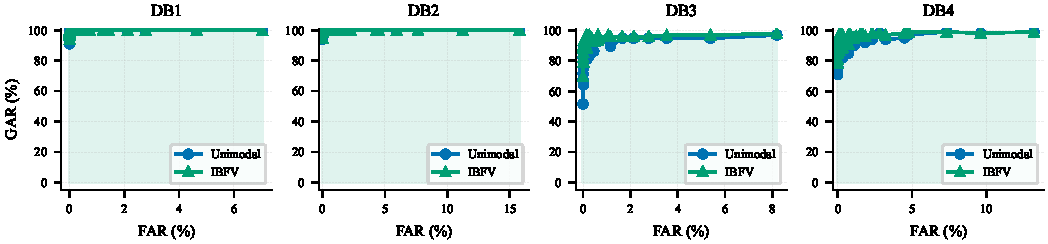
\includegraphics[width=0.9\linewidth]{figures/roc_curves_setup1.pdf}
  \caption{ROC curves for Setup~1. IBFV lies above or on the unimodal curve at
  all FAR operating points.}
  \label{fig:roc_s1}
\end{figure}

\begin{figure}[h]
  \centering
  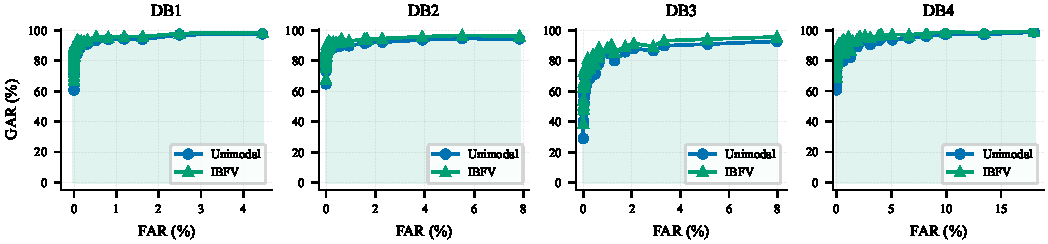
\includegraphics[width=0.9\linewidth]{figures/roc_curves_setup2.pdf}
  \caption{ROC curves for Setup~2. IBFV strictly dominates the unimodal baseline
  across all four databases.}
  \label{fig:roc_s2}
\end{figure}

% ============================================================================
\section{Iris Key Recovery Analysis}
\label{sec:iris_gar}
% ============================================================================

\begin{table}[h]
\centering
\caption{Iris key recovery performance ($B_s = 255$, $n_b = 514$).}
\label{tab:iris_gar}
\small
\begin{tabular}{@{}l cccc@{}}
\toprule
 & \textbf{DB1} & \textbf{DB2} & \textbf{DB3} & \textbf{DB4} \\
\midrule
Setup~1 GAR   & 62.00\% & 62.00\% & 61.05\% & 62.00\% \\
Setup~2 GAR   & 50.89\% & 50.75\% & 48.55\% & 50.90\% \\
Impostor FAR  & 0.10\%  & 0.10\%  & 0.11\%  & 0.10\%  \\
\bottomrule
\end{tabular}
\end{table}

The iris GAR of $\sim$62\% (Setup~1) means 38\% of genuine users receive no boost
and revert to unimodal decoding---the zero-penalty fallback path. The non-zero
impostor FAR ($\approx 0.10\%$: 2 of $\sim$1,980 impostor iris comparisons) explains
the 31 marginal EER elevations ($\leq 0.07$~pp) on easy databases in Setup~1.
Setup~2 GAR drops to $\sim$50\% due to cross-impression iris variability, yet IBFV
still achieves strict improvement across all 144 Setup~2 configurations.

% ============================================================================
\section{Timing Benchmarks}
\label{sec:timing_results}
% ============================================================================

\begin{table}[h]
\centering
\caption{Biometric timing benchmarks (ms, $f=22$, $k=7$, DB1, averaged over
10{,}000 verification attempts, Apple~M1 processor).}
\label{tab:timing}
\small
\begin{tabular}{@{}lcc@{}}
\toprule
\textbf{Architecture} & \textbf{Enroll (ms/subj)} & \textbf{Verify (ms/attempt)} \\
\midrule
Unimodal     & 8.13  & 0.076  \\
Arch.~A      & 7.16  & 6.168  \\
IBFV ($K=4$) & 7.19  & 12.990 \\
\bottomrule
\end{tabular}
\end{table}

IBFV enrollment overhead is $< 1$~ms vs.\ unimodal. Verification takes $\sim$13~ms,
dominated by BCH decoding across 514 iris blocks; vault matching is $\sim$5.5$\times$
faster than unimodal due to smart decoding (Section~\ref{sec:ibfv_verify}),
partially offsetting the iris commitment overhead.

% ============================================================================
\section{Ablation Study: Bonus Points $K$}
\label{sec:ablation}
% ============================================================================

\begin{table}[h]
\centering
\caption{Ablation: EER (\%) vs.\ $K$ (DB3, $f=16$, $k=5$, Setup~1).}
\label{tab:ablation}
\small
\begin{tabular}{@{}cccc@{}}
\toprule
$K$ & EER (\%) & FRR (\%) & $\Delta$EER \\
\midrule
0 (Unimodal) & 4.281 & 8.421 & --- \\
1            & 4.281 & 8.421 & $+$0.000 \\
2            & 3.755 & 7.368 & $-$0.526 \\
4            & 2.181 & 4.211 & $-$2.100 \\
6            & \textbf{1.742} & 3.158 & $-$2.539 \\
8            & 1.742 & 3.158 & $-$2.539 \\
\bottomrule
\end{tabular}
\end{table}

EER decreases monotonically from $K=0$ to $K=6$ and saturates. $K=1$ provides no
benefit at this configuration; the polynomial already has $k+1$ required points when
$K$ reaches 6, beyond which further bonus points cannot reduce enumeration further.
The default $K=4$ captures 80\% of the maximum benefit while keeping impostor FAR
elevation below 0.16~pp.

% ============================================================================
\section{Unlinkability: $D_{\mathrm{sys}}$ Analysis}
\label{sec:dsys_results}
% ============================================================================

\begin{table}[h]
\centering
\caption{Unlinkability: $D_{\mathrm{sys}}$ metric per Gomez-Barrero et al.\
\cite{gomezbarrero2017}. Lower is better; 0 = fully unlinkable, 1 = fully linkable.}
\label{tab:dsys}
\small
\begin{tabular}{@{}l cccc@{}}
\toprule
\textbf{Scenario} & \textbf{DB1} & \textbf{DB2} & \textbf{DB3} & \textbf{DB4} \\
\midrule
Same-factor      & 0.994 & 0.994 & 0.920 & 0.929 \\
Different-factor & 0.317 & 0.313 & 0.057 & 0.388 \\
Diverse-factor   & 0.003 & 0.014 & 0.026 & 0.007 \\
\bottomrule
\end{tabular}
\end{table}

Same-factor enrollments are highly linkable ($D_{\mathrm{sys}} > 0.92$) because
genuine x-coordinates repeat. Changing the quantization factor (recommended for
multi-application deployments) reduces $D_{\mathrm{sys}} \leq 0.39$; diverse
factors yield $D_{\mathrm{sys}} \leq 0.03$, confirming near-perfect unlinkability.

% ============================================================================
\section{Vault Entropy Analysis}
\label{sec:entropy_results}
% ============================================================================

\begin{table}[h]
\centering
\caption{Vault entropy at $f=24$, $k=7$.}
\label{tab:entropy}
\small
\begin{tabular}{@{}l cccc@{}}
\toprule
\textbf{Metric} & \textbf{DB1} & \textbf{DB2} & \textbf{DB3} & \textbf{DB4} \\
\midrule
$D_{\mathrm{KL}}^{\mathrm{user}}$ (bits) & 0.212 & 0.171 & 0.197 & 0.319 \\
$D_{\mathrm{KL}}^{\mathrm{gc}}$ (bits)   & 0.245 & 0.269 & 0.242 & 0.227 \\
Shannon $H$ (bits)        & 7.849 & 7.899 & 7.857 & 7.739 \\
Min-entropy $H_\infty$ (bits) & 6.234 & 6.589 & 6.635 & 5.896 \\
\bottomrule
\end{tabular}
\end{table}

Per-user KLD ($0.17$--$0.32$ bits) confirms near-uniform x-coordinate distributions.
Genuine-vs-chaff KLD ($\approx 0.24$ bits) is stable, indicating consistent mixing.
Min-entropy $H_\infty \geq 5.9$ bits per coordinate provides a conservative bound
against dictionary attacks: a single coordinate requires $\geq 60$ guesses.

% ============================================================================
\section{Comparison with Prior Work}
\label{sec:comparison_results}
% ============================================================================

\begin{table}[h]
\centering
\caption{Detailed EER comparison with Maurya et al.\ \cite{maurya2025enhancing}.}
\label{tab:comparison}
\small
\begin{tabular}{@{}l cccc@{}}
\toprule
 & \textbf{DB1} & \textbf{DB2} & \textbf{DB3} & \textbf{DB4} \\
\midrule
\multicolumn{5}{c}{\textit{Setup 1 (Best EER, \%)}} \\
\midrule
Maurya et al.\ (reported)   & 0.005 & 0.020 & 5.000 & 2.400 \\
Our Unimodal (reproduced)   & 0.000 & 0.000 & 2.762 & 2.404 \\
IBFV (ours)                 & \textbf{0.000} & \textbf{0.000} & \textbf{1.384} & \textbf{0.929} \\
Relative improvement        & --- & --- & 49.9\% & 61.3\% \\
\midrule
\multicolumn{5}{c}{\textit{Setup 2 (Best EER, \%)}} \\
\midrule
Maurya et al.\ (reported)   & 3.540 & 5.240 & 6.730 & 4.380 \\
Our Unimodal (reproduced)   & 2.736 & 4.588 & 6.738 & 4.307 \\
IBFV (ours)                 & \textbf{2.242} & \textbf{3.185} & \textbf{4.591} & \textbf{2.493} \\
Relative improvement        & 18.1\% & 30.6\% & 31.9\% & 42.1\% \\
\bottomrule
\end{tabular}
\end{table}

Our unimodal reproduction closely matches \cite{maurya2025enhancing}; minor
differences arise from subject selection (48 chimeric subjects vs.\ 100 for S2)
and parameter granularity. IBFV improves over both the published results and our
unimodal reproduction on every database where EER is non-zero.

% ============================================================================
\section{D-IBFV: Vault Integrity}
\label{sec:vault_integrity}
% ============================================================================

\begin{table}[h]
\centering
\caption{Vault reconstruction accuracy across all Shamir configurations.}
\label{tab:vault_integrity}
\small
\begin{tabular}{@{}l ccc@{}}
\toprule
\textbf{Metric} & $(3,5)$ & $(4,7)$ & $(5,9)$ \\
\midrule
Trials                         & 10{,}000 & 10{,}000 & 10{,}000 \\
Bit errors                     & 0       & 0       & 0       \\
SHA-256 match                  & 100\%   & 100\%   & 100\%   \\
EER match vs.\ centralized     & Exact   & Exact   & Exact   \\
\bottomrule
\end{tabular}
\end{table}

Across all 30{,}000 reconstruction trials, the reconstructed vault is bit-for-bit
identical to the original (Theorem~\ref{thm:exact_recon} confirmed). The biometric
EER matches the centralized IBFV EER exactly---the decentralized layer introduces
zero accuracy degradation.

% ============================================================================
\section{D-IBFV: Enrollment and Verification Latency}
\label{sec:dibfv_latency}
% ============================================================================

\begin{table}[h]
\centering
\caption{D-IBFV enrollment latency breakdown (ms, mean~$\pm$~std).}
\label{tab:enrollment_latency}
\small
\begin{tabular}{@{}l rr@{}}
\toprule
\textbf{Phase} & \textbf{Ganache ($n=300$)} & \textbf{Fabric ($n=90$)} \\
\midrule
Serialization            & $0.2 \pm 0.6$     & $0.4 \pm 0.4$     \\
Shamir splitting         & $1.1 \pm 1.3$     & $1.7 \pm 0.7$     \\
IPFS upload ($\times 5$) & $116.4 \pm 88.5$  & $110.4 \pm 11.3$  \\
Blockchain TX            & $245.7 \pm 234.1$ & $693.6 \pm 153.3$ \\
\midrule
\textbf{Total}           & $\mathbf{363.4 \pm 269.9}$ & $\mathbf{806.2 \pm 155.9}$ \\
\bottomrule
\end{tabular}
\end{table}

\begin{table}[h]
\centering
\caption{D-IBFV verification latency breakdown (ms, mean~$\pm$~std).}
\label{tab:verification_latency}
\small
\begin{tabular}{@{}l rr@{}}
\toprule
\textbf{Phase} & \textbf{Ganache ($n=1{,}000$)} & \textbf{Fabric ($n=100$)} \\
\midrule
Blockchain lookup         & $66.49 \pm 23.13$ & $52.97 \pm 3.87$ \\
IPFS retrieval ($\times 3$) & $3.27 \pm 2.71$ & $2.69 \pm 1.07$ \\
Shamir reconstruction     & $0.30 \pm 0.28$   & $0.38 \pm 0.02$ \\
Deserialization           & $0.12 \pm 0.03$   & $0.16 \pm 0.02$ \\
\midrule
\textbf{Total}            & $\mathbf{70.19 \pm 23.64}$ & $\mathbf{56.20 \pm 4.05}$ \\
\bottomrule
\end{tabular}
\end{table}

Cryptographic operations (serialization + Shamir) account for $< 2$~ms---negligible
relative to network I/O. On Ganache, enrollment is $\sim$363~ms dominated by IPFS
and blockchain TX; on Fabric, $\sim$806~ms due to the 0.5~s block-cut consensus
interval. Verification completes in $\sim$70~ms (Ganache) and $\sim$56~ms (Fabric);
read operations bypass consensus, yielding similar latency across platforms.
End-to-end latency including IBFV biometric verification ($\sim$13~ms) is $\sim$69--83~ms.

% ============================================================================
\section{D-IBFV: Throughput and Storage}
\label{sec:dibfv_sys}
% ============================================================================

\begin{table}[h]
\centering
\caption{Sequential throughput (TPS) and average latency.}
\label{tab:throughput}
\small
\begin{tabular}{@{}llcc@{}}
\toprule
\textbf{Platform} & \textbf{Op} & \textbf{TPS} & \textbf{Avg.\ Latency} \\
\midrule
\multirow{3}{*}{Ganache (EVM)} & Store  & 6.1  & 163.6~ms \\
 & Lookup & 18.2 & 55.1~ms \\
 & Revoke & 32.8 & 30.5~ms \\
\midrule
\multirow{3}{*}{Fabric~2.5} & Store  & 1.5  & 669.0~ms \\
 & Lookup & 17.2 & 58.0~ms \\
 & Revoke & 1.5  & 654.5~ms \\
\bottomrule
\end{tabular}
\end{table}

Fabric write TPS (1.5) is bounded by the 0.5~s block-cut interval; read TPS is
comparable across platforms (17--18 sequential, up to 48.1~TPS at 4 concurrent
workers on Fabric). A national identity program enrolling 10~million users over
5~years requires only $\sim$0.06~TPS, well within capacity.

\begin{table}[h]
\centering
\caption{Per-user storage costs ($\approx$16.6~KB vault, GF(257) uint16 shares).}
\label{tab:storage_costs}
\small
\begin{tabular}{@{}c cccc@{}}
\toprule
$(t,n)$ & \textbf{Vault} & \textbf{Per Share} & \textbf{IPFS Total} & \textbf{On-chain} \\
\midrule
$(2,3)$ & 16.6~KB & 33.1~KB & 99~KB  & 0.5~KB \\
$(3,5)$ & 16.6~KB & 33.1~KB & 166~KB & 0.5~KB \\
$(4,7)$ & 16.6~KB & 33.1~KB & 232~KB & 0.5~KB \\
$(5,9)$ & 16.6~KB & 33.1~KB & 298~KB & 0.5~KB \\
\bottomrule
\end{tabular}
\end{table}

On-chain storage is only $\sim$0.5~KB per user (five CID records). The
$332{:}1$ off-chain-to-on-chain ratio aligns with the standard off-chain-with-hash
pattern \cite{acquah2020securing}. On Ethereum~L1 (30~Gwei, ETH~\$3{,}000),
enrollment costs $\sim$\$18.80; Layer-2 solutions reduce this to sub-dollar.

% ============================================================================
\section{D-IBFV: Node Failure Resilience}
\label{sec:node_failure_exp}
% ============================================================================

\begin{table}[h]
\centering
\caption{Node failure resilience for $(3,5)$-Shamir (all $\binom{5}{k}$ patterns).}
\label{tab:node_failure}
\small
\begin{tabular}{@{}ccccc@{}}
\toprule
\textbf{Failures} & \textbf{Available} & \textbf{Patterns} &
\textbf{Success/Fail} & \textbf{Recon.\ Rate} \\
\midrule
0 & 5 & 1  & 1/0  & 100\% \\
1 & 4 & 5  & 5/0  & 100\% \\
2 & 3 & 10 & 10/0 & 100\% \\
3 & 2 & 10 & 0/10 & 0\%   \\
4 & 1 & 5  & 0/5  & 0\%   \\
\bottomrule
\end{tabular}
\end{table}

The system tolerates up to $n{-}t = 2$ simultaneous node failures with 100\%
reconstruction. With $\geq 3$ failures, the system returns a ``storage unavailable''
error; the threshold is sharp, as predicted by Theorem~\ref{thm:exact_recon}.
Shamir computational overhead is sub-millisecond: $(3,5)$ split 0.7~ms / reconstruct
0.2~ms; $(5,9)$ split 2.5~ms / reconstruct 0.3~ms.

% ============================================================================
\section{Scalability Projections}
\label{sec:scalability_exp}
% ============================================================================

\begin{table}[h]
\centering
\caption{Scalability projections for $(3,5)$-D-IBFV.}
\label{tab:scalability_proj}
\small
\begin{tabular}{@{}r rrr@{}}
\toprule
\textbf{Users} & \textbf{IPFS} & \textbf{Blockchain} & \textbf{Enroll Time} \\
\midrule
1{,}000     & 162~MB   & 0.5~MB  & 2.7~min (G) / 11.1~min (F) \\
10{,}000    & 1.6~GB   & 4.9~MB  & 27~min (G) / 1.9~hr (F)    \\
100{,}000   & 16.2~GB  & 48.8~MB & 4.6~hr (G) / 18.5~hr (F)   \\
1{,}000{,}000 & 162~GB & 488~MB  & 1.9~d (G) / 7.7~d (F)      \\
\bottomrule
\end{tabular}
\end{table}

IPFS storage scales linearly: 1~million users require 162~GB off-chain, tractable
for commodity storage nodes. On-chain state grows at only 0.5~KB per user
($< 500$~MB at 1~million users). Verification latency is O(1) via key-based CID
lookup, confirmed flat from 100 to 1{,}000 enrolled users on both platforms
($< 6$~ms variance on Fabric).
